
Symbols are geometry with meaning.  The symbol is perhaps the most general idea that exists in human thought, since everything we do is mediated through the use of some type of symbol.  When we speak of symbols in Geometron we mean \emph{any} geometric construction which has meaning to people.  This includes not written language like text but constructions like the layout of a microchip or the design of a building.  It also includes the way we control machines, how we program them build automation. Geometron represents a new framework for working with all these kinds of symbols.  

We live in a civilization today totally dominated by numbers and by the people who work with numbers.   The machines we currently use to communicate are built by people who believe that the most fundamental task such machines can do is to work with numbers.  They call all these machines ``computers'' and have a whole theoretical framework for understanding how to build them using the ideas of arithmetic.  This works. But it is extremely inefficient and distracts from the real purpose of such machines.   Do these machines do arithmetic? Of course.  They also keep very accurate time, does that make them clocks? They produce heat, does that make them heaters?  No.  Just as we don't call a light bulb a ``screw'' just because it screws into a socket, it does not make sense to let the idea of the arithmetic engine dominate in a technology the sole purpose of which is to communicate with other people using symbols.  At some intuitive level, most people understand this, it is why the smart phone is primarily called a ``phone'' rather than a ``computer''.  But the underlying mathematical constructs which built the digital computer remain, along with a whole lot of mathematical flotsam and jetsam which have held back progress and made simple and free media out of reach.
 
In Geometron we are switching from a world view based on numbers to one based on geometry.  This represents a shift in value system.  In ``computer science'', the manipulation of numbers and logic are considered the most fundamental operations.  In Geometron, we consider geometric constructions to be the most fundamental.  This is a shift in perspective, which we can apply to the whole of the existing machines.  How are these machines built? The microchips which make them work are nothing but huge geometric constructions, made up of little overlapping rectangles and polygons.  These chips are then laid out on circuit boards which are again geometric constructions.  The chips are placed automatically on the boards using machines programmed to carry out a sequence of geometric motions.   They are packaged in cases made in molds again machined with this kind of geometric programming. And finally when assembled, their main task is displaying symbols on the screen which is again just geometric construction.   

It is easy to forget given the onslaught of propaganda from Silicon Valley just how accidental the rise of their machines as the dominant technology was.  We also are encouraged to forget that these machines were built \emph{primarily} for war initially, then large authoritarian organizations to track and control people, and only later, almost as an afterthought, as the communication devices we rely on for all aspects of modern life.  One of the theses of Geometron is that a shift in thinking from one based on numbers to one based on geometry is a shift away from the ideology of dominating large amounts of land and people toward one of cooperation based on sharing of technology and ideas.  

When we build everything from trash found directly in our environment, empire-building doesn't really accomplish anything.  The people 1000 miles away from you have the same piles of broken phones you do, so you gain nothing by dominating them and vice versa.  But if you can share with them how to make those phones part of your free network, the value of \emph{your} network infrastructure goes up exponentially, just as we find in all networks. as they scale up.  
  
In computer science, they work with an idea called a Turing Machine, named after computer pioneer Alan Turing, which is a generalized machine for doing arithmetic.  An infinite tape of ones and zeros is fed into this imaginary machine, and the contents of that tape give instructions to the machine, which then carries out actions on the ones and zeros on the tape.  Any computer, regardless of the details of how it is built, can be shown to be equivalent to this toy model.  In Geometron, we are creating a similar object: an abstraction which can construct any symbol, which takes symbols as an input.  

The basis of geometric programming in Geometron is the Geometron Virtual Machine, or GVM.  Just like the Turing Machine, this is an abstract construct which carries out geometric constructions based on a set of instructions.  We assume that there is a main program, which we call a ``glyph'', which consists of a sequence of symbols, each of which represents a geometric action.  Just as the Turing machine reduces every math problem to binary arithmetic, our machine reduces all geometry to discrete geometry.  The GVM has an internal geometric state which represents its progress in doing geometric actions.  If we are programming a physical machine like a pen on a plotter, the position of the pen is stored this way.  This logic is very similar to that of languages like Logo, a teaching language developed in the 1970s, which uses what is called ``turtle logic'', where patterns are drawn by a virtual turtle which moves around on a screen, and which can also be performed by a physical robot with a pen.  However what we are doing differs radically from Logo as we will see below.

We also have states of this virtual machine which describe what motions it can carry out.  The most basic of these is the step size.  By creating geometric programs using an abstract step size without actual numbers, we can create programs to draw symbols independent of what machine we use and what scale we are at, copying verbatim a program from a giant wall climbing robot which spray paints symbols on a building to a nanolithography system which prints the exact same symbol in an area smaller than a human hair, without ever dealing with the mechanism of either machine.  This unit state is also used to define how we do constructions like ``draw a circle''.  

The most basic geometric program we can carry out is the construction of the Vesica Piscis.  This figure, from the Latin ``fish bladder'', is just two circles each of which has its center along the edge of the other.  In the dialect of Geometron presented here, the symbols are all printed inside squares of identical size, patterned from left to right.  The symbol describing the action of drawing a circle is a square with a circle in it, and that draws a circle with radius equal to the current value of the step size.  If we draw a circle of radius equal to step size, then move sideways one unit of that same step size and repeat the action, we get the Vesica Piscis. The symbol to move to the side is just an arrow pointing to he side.  These symbols are themselves constructed using more of the actions of Geometron: drawing line segments, rotating by discrete angles, scaling the unit down and back up and so on.

\begin{figure}
	\centering
	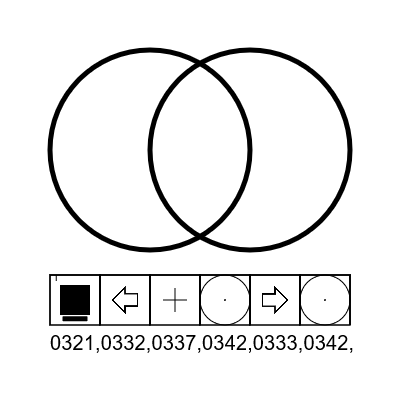
\includegraphics[width=3in]{figures/symbol/vesicapiscisspelling.png}
	\caption[vesicapiscis]
	{Vesica piscis, or ``fish bladder'' spelled out with Geometron symbol glyphs.}
\end{figure}

Another central organizing principle of Geometron is that there are special symmetries and scales that are intrinsic to the Universe which we use to simplify how we approach geometry.  In a numbers-driven system, coordinates and angles are all equal.  37.34 degrees is no different than 36 degrees for example, they are just different numbers with no special properties.  But this ignores some very deep patterns in how the world around us functions.  Both the natural world and the constructed world of human technologies rely constantly on special rotational symmetries, starting with small numbers of rotations, in particular twofold, threefold, fourfold, fivefold, sixfold, eightfold, tenfold, and twelve fold.  From there if we add halving angles and dividing them by 3 we can get all the way to the 360 fold symmetry which defines the degree of angular measure in most common use.  Using only discrete geometric manipulations, we can go from fivefold symmetry which is based on 72 degrees, divide by 2 to get 36 degrees, then divide by 3 three times to get 1 degree.  So discrete geometric actions can be used to do a very wide range of geometric constructions without ever relying on reference to numerical representations of angles.  The dialect of Geometron presented is based primarily on 4,5, and 6 fold symmetry, combined with halving, doubling, dividing by three, and multiplying by three to construct all angular rotation actions. 

By default, we increase or decrease our unit of step movement and construction by factors of two.  Just like in digital computers, this binary representation allows us in principle to represent any number using only geometric actions of doubling, halving and moving by discrete amounts.  Again this allows us to program a machine to go to any coordinate without actually using numbers, only using symbols which represent geometric actions.  Those could all be represented by numbers of course, but we choose to \emph{express} them using pure geometric symbols.  And just as binary arithmetic can express any number, this binary geometry can express every position in space.

Another intrinsic geometric property we find in the world around us is the scales which naturally go along with these symmetries.  For example, when we deal with fivefold symmetry, everything is based on the Golden Ratio.  The ratio of the side of a regular pentagon to the distance along the cords which make up a pentagram drawn inside it is this ratio.  If we then build a fractal of pentagrams inside pentagrams, the way we scale down to smaller and smaller pentagrams and pentagons is again and again the Golden Ratio.  This number is about 1.6 and is a universal constant built into the structure of the Universe, found in all kinds of natural systems, as well as used throughout human art, architecture, and technology.  While a numbers-based system can of course compute geometry using this number expressed as a repeating decimal, in Geometron we simply use a symbol to represent this scale, without any symbolic reference to its numerical value.  

\begin{figure}
	\centering
	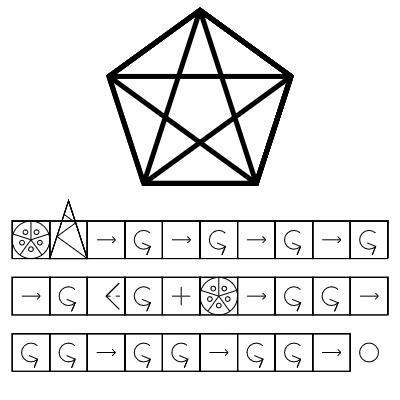
\includegraphics[width=3in]{figures/symbol/pentagram.png}
	\caption[pentagram]
	{The pentagram in a pentagon, showing the relationship between the Golden Ratio and fivefold symmetry.}
\end{figure}


The square root of three plays a similar role to the Golden Ratio, but for sixfold symmetry.  If one connects alternating corners of a regular hexagon, those cords are the square root of three times the length of a side.  Again, a fractal construction of hexagons and six pointed stars shows a square root of three scaling over and over.  Similarly, the square root of two is intrinsic to four fold symmetry, as if we draw a diagonal line across a square that is the square root of two times the side length.  

\begin{figure}
	\centering
	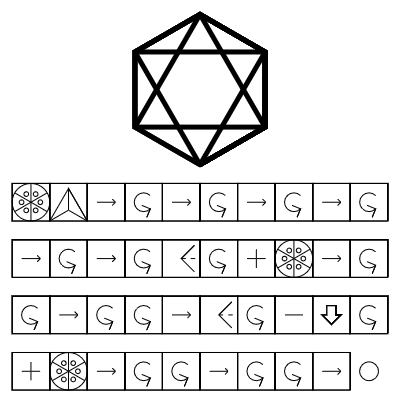
\includegraphics[width=3in]{figures/symbol/hexagram.png}
	\caption[hexagram]
	{The six pointed star in a hexagon, showing the relationship between the square root of three and sixfold symmetry.}
\end{figure}

\begin{figure}
	\centering
	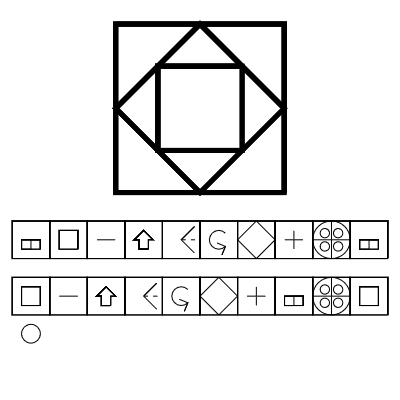
\includegraphics[width=3in]{figures/symbol/squareroottwo.png}
	\caption[squareroottwo]
	{Embedded squares showing the relationship between four and eight fold symmetry and the square root of two.}
\end{figure}

Altogether, the scales used in this dialect are, in order, the square root of two, the Golden Ratio, the square root of three, 2, 3, and 5.  When a scale is set, that scale is the factor by which the unit is either multiplied or divided when we apply a scale-up or scale-down operation.  


\begin{figure}
	\centering
	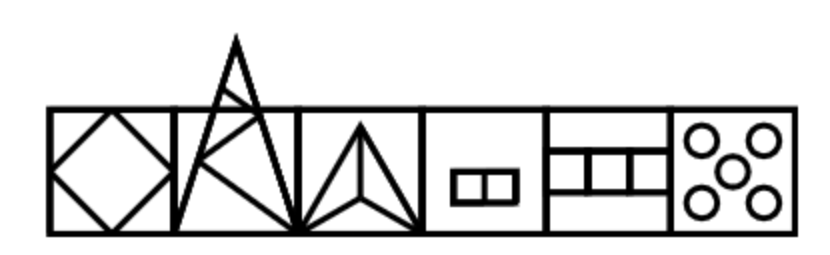
\includegraphics[width=3in]{figures/symbol/scales.png}
	\caption[scales]
	{Scale actions in order: square root of two, Golden Ratio, square root of three, two, three, five.}
\end{figure}


The figures show the symbols for all these scale values.  We are now ready to understand all 8 of the basic discrete movements: move forward, move back, move left, move right, rotate left, rotate right, scale down and scale up.     

The current state of the GVM is expressed with the Global Cursor, a shape which shows the position, scale, the step angle size, the current direction which is ``forward'' and the current directions which are ``left'' and ``right''.

\begin{figure}
	\centering
	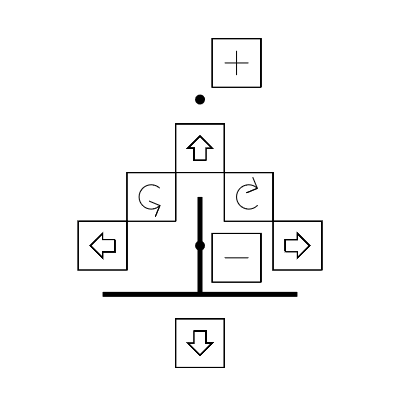
\includegraphics[width=3in]{figures/symbol/cursormovements.png}
	\caption[cursormovements]
	{GVM cursor with movements. The arrows represent movement of the GVM position along the indicated directions relative to the cursor.  Angle rotations are as shown.  The plus and minus symbols are also shown and how the rescale to where the points are on the cursor.}
\end{figure}



The basic constructions of Geometron are to draw a point at the current location, draw a circle of radius equal to the current unit, draw a line segment along the forward direction, and draw an arc from one of the cursor wings to the other.  More advanced actions include writing letters, creating paths(both filled and unfilled, closed and open), and drawing Bezier curves, all of which will be covered in the next, more detailed section on the web-based graphics system which is built into Geometron.

Color and line width of lines are set with the layer system.  At any given point along the construction of a Geometron glyph, one of the states is the current layer, of which there are 8. Each layer has a stroke color, a fill color, and a line width.  These are set in an object which can be edited and customized, which the GVM calls on when it draws symbols.

\begin{figure}
	\centering
	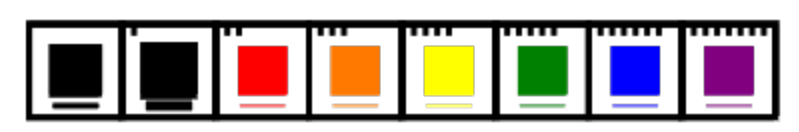
\includegraphics[width=3in]{figures/symbol/colors.png}
	\caption[colors]
	{Symbols for the layers have little line segments to denote the layer number, and show the line width, fill colors and stroke colors in the border and fill of squares.}
\end{figure}

  
A very important point to make about how all this fits together is that each of the symbols shown here which represent these geometric actions are themselves constructed using this language.  When a symbol is displayed in the spelling out of a Geometron glyph, each of the actions which compose the glyph has a symbol which is itself a Geometron glyph, and the whole sequence of symbols which spells out the glyph is itself one giant glyph which tells the GVM how to spell out this human readable symbolic description.  

\begin{figure}
	\centering
	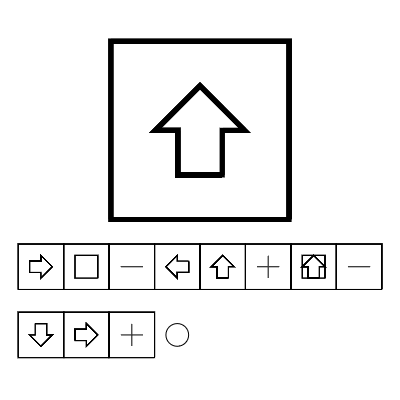
\includegraphics[width=3in]{figures/symbol/uparrowspelling.png}
	\caption[uparrowspelling]
	{Breaking a symbol glyph down into its constituent action glyphs.  This shows the spelling for the geometric action which moves forward one unit.  It includes a sub-action which draws the arrow.}
\end{figure}



Geometron glyphs consist of a sequence of geometric actions.  Each action has a symbol, which is itself made up of actions, each of which has a symbol and so on(recall that one of the laws of Geometron is that everything is recursive). Each geometric action is represented by an address in the Geometron Hypercube.  The Hypercube consists of two cubes, each divided into 8x8x8 = 512 cells, for a total of 1024 cells.  Each cell contains a glyph, which is itself a sequence of addresses in the Hypercube.  The Hypercube is therefore a kind of recursive data structure, with many components which all point back to itself.  It might be added that human languages are all forms of recursive data structure, as they are described using the language itself(e.g.dictionaries).  Hypercube addresses consist of four digits each of which is a number between 0 and 7, and the first digit of which is 0 or 1, just denoting what cube it in.

Why, you might ask, do we add this complexity?  It is deceptively powerful to create a structure like this.  Note that this structure is completely geometric.  While we emph{represent} each cell with numerical addresses, the actual underlying structure is geometric and symbolic.  Elements represent geometric symbols, human language describing geometry, computer language describing geometry,  and locations in a data space.  This is a non-numerical construct, and represents a fundamental shift from the Turing model of computers to a model for a generalized symbol constructor.  If our goal in building technology is to draw symbols, our fundamental models should reflect this, and not mask it in ``computation''.  

\begin{figure}
	\centering
	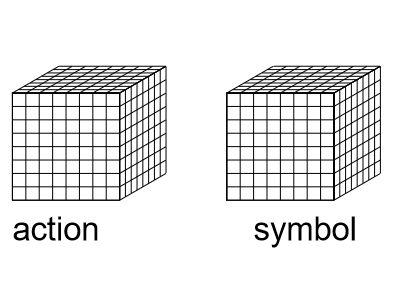
\includegraphics[width=3in]{figures/symbol/cubes.png}
	\caption[cubes]
	{The two Cubes of the Geometron Hypercube: the Action Cube and the Symbol Cube.}
\end{figure}


Of the two cubes in the Hypercube, one is the ``action cube'' and the other is the ``symbol cube'', which has a leading 1 in the 4 digit address instead of 0.  Each action in the action cube therefore has a corresponding symbol.  Thus when a GVM is spelling out a sequence of symbol glyphs, it is just carrying out the actions represented by addresses of the form 01xyz, which are in turn simply doing the list of actions stored in that address in order.  Any time you see Geometron symbol glyph spelling, you are looking at a sequence of symbol cube addresses.

But what of the Action Cube?  This has a lot more structure than just all being actions.  As said above, we are looking to build a geometric language which can apply to the widest possible range of generalized symbols. This means we want to be able to not only make 2d symbols, but to make complex fractal structures of symbols made from symbols for specialized graphics, printing in any human language, 3d constructions, editing the hypercube itself and perhaps most importantly machine control for generalized automation.

The Action Cube's bottom addresses from 0 to 037 represent actions directly on the Hypercube and the GVM and environment. These are used for tasks like moving the cursor around, choosing which element of the Hypercube is being edited, deleting addresses from a glyph, and changing the view geometry of the symbol display(zoom and pan).

Addresses from 040 through 0176 represent the printable characters on the standard keyboard using the ASCII code.  These addresses all map to actions which are carried out when that key is struck on a keyboard.  These are physical inputs.  They are geometric in the sense that keyboards are geometric, and that hitting keys is a geometric action.  The corresponding symbols stored in the Symbol Cube at 01040 through 01176 represent a font.  These can be any kind of character, and can be used for any keyboard mapping to any human language.  This represents an alternative to Unicode, in which each glyph is directly created using the Geometron langauge, rather than called from the system's interpretation of Unicode.

Address 0177 represents ``do nothing'' and can be empty or used as a dummy variable.

The addresses between 0300 and 0377 are the two dimensional actions described above and in the next chapter, which are used for making web graphics, saved vector graphics files, and all the symbols used to represent Geometron glyphs.  These are in practice all some type of computer function call, and since computer code is stored in ASCII and ASCII is part of the Hypercube, these little bits of code represent the sequence of Hypercube addresses which can be represented as a sequence of ASCII codes which can map to addresses in the Hypercube, so we retain our generalized structure. Also, if we take this as a total abstraction, we could describe the geometric action using text in a human language, such as ``draw circle of unit radius'', and that can be encoded in ASCII to make it part of the Hypercube format as well. 

The addresses from 0200 through 0277 are the ``Shape Table'' and all store sequences either in 02xy as well or in the range of 03xy.  This is merely a convention, but these are used to build up specialized language, such as for building circuit diagrams or cross stitch patterns.  This topic has its own chapter, as there is a very rich range of languages which we can build this way.

Addresses between 0400 and 0477 represent machine actions.  The most basic actions for machines we consider are for machines that have 3 perpendicular axes of movement, of which we have several examples later in this work.  Using only the actions of discrete movement and binary manipulation on the scale of the step, this system can be used to encode any motion of a robotic probe, but that only takes up one row of 8 out of the total of 64 possible actions.  This is also a topic so rich in structure that it has its own chapter.  The ability to use a web interface to do totally generalized programming of the geometry of machines for automation can revolutionize the control humans have over machines and over automation.  

Addresses between 0500 and 0577 are another shape table, specifically for referencing machine actions in 04xy.  As with all Shape Tables, this can be self-referential, and we can use this space to build up fractal structures of motions within motions.  This can be a huge enabling technology for programming of automation using simple machines.  The actions in this range are used to create a form of generalized ``icon'', which also gets its own chapter.  Icons are sequences of movements on a rectangular grid, which either involve drawing a pixel or not.  This sequence is used to create physical media using a variety of technologies, which are documented in the aforementioned chapter.  

Finally, the addresses at the top of the Action Cube from 0700 through 0777 represent three dimensional constructions.  These are abstract, and can be applied to any method of three dimensional construction.  These also get their own chapter, and can be used to create graphics in the virtual reality format of x3d as well as .stl files which can be printed on a 3d printer.  They are displayed in the browser live using webGL libraries discussed later on.  The Shape Table at 0600 through 0677 is for calling actions in the 07xy cube, for building up complex fractal structures in 3d construction.  This can server as the basis of a whole alternative system for creating parts for 3d printing, as well as a basis for web-based 3d graphics for both virtual reality and augmented reality.
   
The structures described here, the GVM and the Geometron Hypercube, represent a new way of thinking about how humans control machines.  In this way of thinking, the purpose of machines is to encode geometric information on the physical world in a way which communicates information to another human being.  We start with this as a goal and build up a set of abstractions to do that as generally as possible.  Just as the Turing Machine toy model has been implemented in vastly different physical systems, our abstract idea about symbol drawing machines can take totally different forms which carry out the same task as well.  This is a key element of how we will build the hybrid trash-based hardware architecture described later in this work.  We do not want to compute things. We want to display symbols and images on screens, and control the movements of the machines we build from trash to automate building more things from trash. That is all.  If we can display a generic geometric symbol on a scavenged screen, we can create fully Organic Media as described in an earlier chapter.  That is, media which self-replicates openly on a physical network, which needs no mined materials, no money, and no property.  If this is easy and uses trashed cell phones, the constant stream of broken phones will allow us to create a model of ubiquitous networking of Organic Media by way of the Street Network.  With the consumer based system creating billions and billions of phones all headed to the landfill, we can imagine a model where there are screens everywhere, but they're not mobile because they don't need to be.  In a network with self-replicating documents, you can read what documents you want wherever you go.  You can interact with a universe of documents which flows through the physical world, as you traversethat world, interacting with and improving documents as you go as you interact with people in the physical world.    The hardware architecture to realize this will be discussed in its own chapter on Full Stack Geometron.


\begin{figure}
	\centering
	
\includegraphics[width=3in]{figures/shapes/blank.png}
\end{figure}
\begin{figure}
	\centering
	
\includegraphics[width=3in]{figures/shapes/blank.png}
\end{figure}
\begin{figure}
	\centering
	
\includegraphics[width=3in]{figures/shapes/blank.png}
\end{figure}
